\documentclass[11pt]{article}
\usepackage[margin=1in]{geometry}
\usepackage[T1]{fontenc}
\usepackage[utf8]{inputenc}
\usepackage{lmodern}
\usepackage{amsmath,amssymb,booktabs}
\usepackage{graphicx}
\usepackage{microtype}
\usepackage[hidelinks]{hyperref}
\usepackage{xurl}
\setlength{\emergencystretch}{3em}
\graphicspath{{../notes/build/}}

\title{Fertility, Baby Booms, and the Political Economy of Housing Supply}
\author{Draft}
\date{March 20, 2026}

\begin{document}
\maketitle

\begin{abstract}
This paper studies how adding fertility to a political-economy model of housing supply changes the
mapping from demographics to house prices. The baseline environment is the NIMBY housing-supply
framework: households vote over local supply through the effect of house prices on lifetime
utility. The fertility extension preserves that political and real-estate structure but augments
the household problem with births, children at home, and crowding. Four quantitative results
emerge. First, in the steady-state benchmark, the fertility channel shifts political support
toward lower house prices: the equilibrium crossing falls from 2.326 in the NIMBY benchmark to
1.752 in the fertility benchmark. Second, a temporary baby boom produces a larger medium-run house
price response in the fertility model than in the NIMBY benchmark because children at home raise
current housing-space demand. Third, the same fertility margin improves the fit to the postwar
decline in aggregate fertility after the baby boom, although the improvement is modest. Fourth,
when the demographic change comes from projected long-run aging rather than a temporary child
wave, the fertility channel dampens the rise in house prices relative to the NIMBY proxy. The
paper is therefore not ``NIMBY plus one more block.'' It is a model of how family formation
changes both the short-run and long-run political economy of housing supply.
\end{abstract}

\section{Introduction}

The starting point of this paper is the NIMBY housing-supply model. In that framework, households
vote over local supply through the way a small persistent change in house prices affects expected
lifetime utility. The core political mechanism is clear: younger households and marginal future
buyers tend to prefer lower prices, while older owners tend to prefer higher prices. Demographic
change therefore matters because it changes the composition of the electorate.

This paper asks what changes once fertility is added to that environment. Housing matters for
family formation in a way that is absent from the original NIMBY benchmark. A birth does not just
change the future size of a cohort. It also changes current housing demand because children at
home make crowding costly. High house prices can therefore discourage births, while a temporary
baby boom can tighten current demand for housing space. Those forces do not replace the original
NIMBY mechanism. They interact with it.

The central claim is simple. Adding fertility changes the sign and timing of demographic pressure
in the housing market. In the steady state, the fertility channel makes high house prices less
politically acceptable because family-forming households care about both housing costs and
crowding. In a temporary baby boom, however, the same fertility channel raises current demand for
space and amplifies the medium-run house-price response. Under projected long-run aging, by
contrast, the family channel works in the opposite direction: as the mass of family-forming
households falls, the fertility extension tempers the aging-driven rise in house prices implied by
the baseline NIMBY mechanism.

The paper is organized around that comparison. Section 2 sets out the model and isolates exactly
what changes relative to the NIMBY benchmark. Section 3 reports the steady-state benchmark.
Section 4 studies a temporary baby boom. Section 5 compares the model's post-boom fertility path
to the postwar decline in US fertility. Section 6 shows that the short-run price result is robust
to a bounded set of parameter changes. Section 7 turns to projected demographic aging. Section 8
concludes.

\section{Model}

\subsection{Baseline environment}

The baseline environment is the NIMBY housing-supply framework. Households live through the life
cycle, consume non-housing goods and housing services, and vote over local supply through the
effect of a small house-price change on expected lifetime utility. Real-estate firms supply
housing competitively. The local political equilibrium is determined by a median-voter condition.

What this paper changes is the household problem, not the political equilibrium concept. The
fertility model keeps the same house-price object, the same political tightness object, and the
same logic through which demographics shift the voting schedule. The difference is that family
states now enter utility and state transitions directly.

\subsection{Household problem}

In the NIMBY benchmark, a household's state consists of liquid assets, housing position, and
income state. In the fertility model, that state is augmented with two family variables:
\begin{enumerate}
\item parity, or children ever born;
\item children currently at home.
\end{enumerate}

That distinction matters. Completed fertility is permanent. Crowding is temporary. A household can
have several children over its life cycle without having all of them at home at once.

The key utility change is that housing enters through effective housing services rather than raw
housing services:
\begin{equation}
H_t^{eff} = \frac{H_t}{(1+\lambda_c h_t)^{\psi_c}},
\end{equation}
where $h_t$ is the number of children currently at home. Children therefore lower the effective
amount of housing space available to the household.

Absent a birth, the flow utility in the fertility extension is
\begin{equation}
u_t^{F,0} = \log c_t + s_h \log H_t^{eff} + \nu_h h_t - \text{penalty}_t.
\end{equation}
With a birth, the newborn counts immediately in both the crowding state and the family-utility
term:
\begin{equation}
u_t^{F,1} = \log c_t + s_h \log\left(\frac{H_t}{(1+\lambda_c(h_t+1))^{\psi_c}}\right)
+ \nu_h(h_t+1) + \phi(p_t) - \kappa_0 - \kappa_q q_t - \text{penalty}_t.
\end{equation}
Here $\phi(p_t)$ is parity-specific birth utility, $\kappa_0$ is a direct birth cost, and
$\kappa_q q_t$ is a house-price-sensitive birth cost.

This immediately implies two new margins that are absent from the NIMBY benchmark. First, high
house prices discourage births directly through the birth-cost term. Second, they discourage
births indirectly because a child makes crowding more costly when housing is scarce. Those are the
channels that connect fertility to housing politics.

\subsection{Political equilibrium}

The political block is unchanged in form. A household supports tighter supply when a small
persistent increase in the house price raises expected lifetime utility. Aggregating those
household preferences across the stationary distribution yields the median-voter condition that
pins down the equilibrium house price.

So the fertility model does not introduce a new political mechanism. It changes the object being
fed into the old one. Because the value function now depends on family state, the same price
perturbation is evaluated differently by otherwise similar households at different points of the
family life cycle.

\section{Steady-State Benchmark}

The first benchmark fact is exact nesting. When the fertility block is shut off, the fertility
solver reproduces the upstream NIMBY benchmark exactly. That is important because it means the
comparison is not being driven by a different political closure, a different real-estate block, or
a different equilibrium definition.

With fertility active, the benchmark changes materially. Table \ref{tab:benchmark} summarizes the
main steady-state comparison. The key result is that the equilibrium crossing shifts toward lower
house prices. In the upstream NIMBY benchmark, the crossing occurs at 2.326. In the fertility
benchmark, it occurs at 1.752.

\begin{table}[htbp]
\centering
\caption{Steady-state benchmark comparison}
\label{tab:benchmark}
\begin{tabular}{lcc}
\toprule
Object & NIMBY benchmark & Fertility benchmark \\
\midrule
Crossing house price & 2.326287 & 1.751853 \\
Vote at refined price & 0.002227 & 0.008446 \\
Vote per unit mass at refined price & 0.000349 & 0.001370 \\
Stationary household mass & 6.387684 & 6.163346 \\
Average birth rate & -- & 0.597710 \\
\bottomrule
\end{tabular}
\end{table}

The interpretation is straightforward. In the NIMBY benchmark, house prices matter through tenure
and portfolio position. In the fertility model, they also matter because family-forming
households care about crowding and because births become more expensive when housing is costly.
That additional family margin makes high prices less politically attractive.

Figure \ref{fig:steady_state_support} shows the state-level support schedules behind that result.
The NIMBY logic is still visible. Young households are less supportive of high prices than older
owners. But the fertility extension rotates the support schedule downward for family states that
carry children at home. Figure \ref{fig:steady_state_objects} shows the aggregate benchmark
objects on the common house-price grid.

\begin{figure}[htbp]
\centering
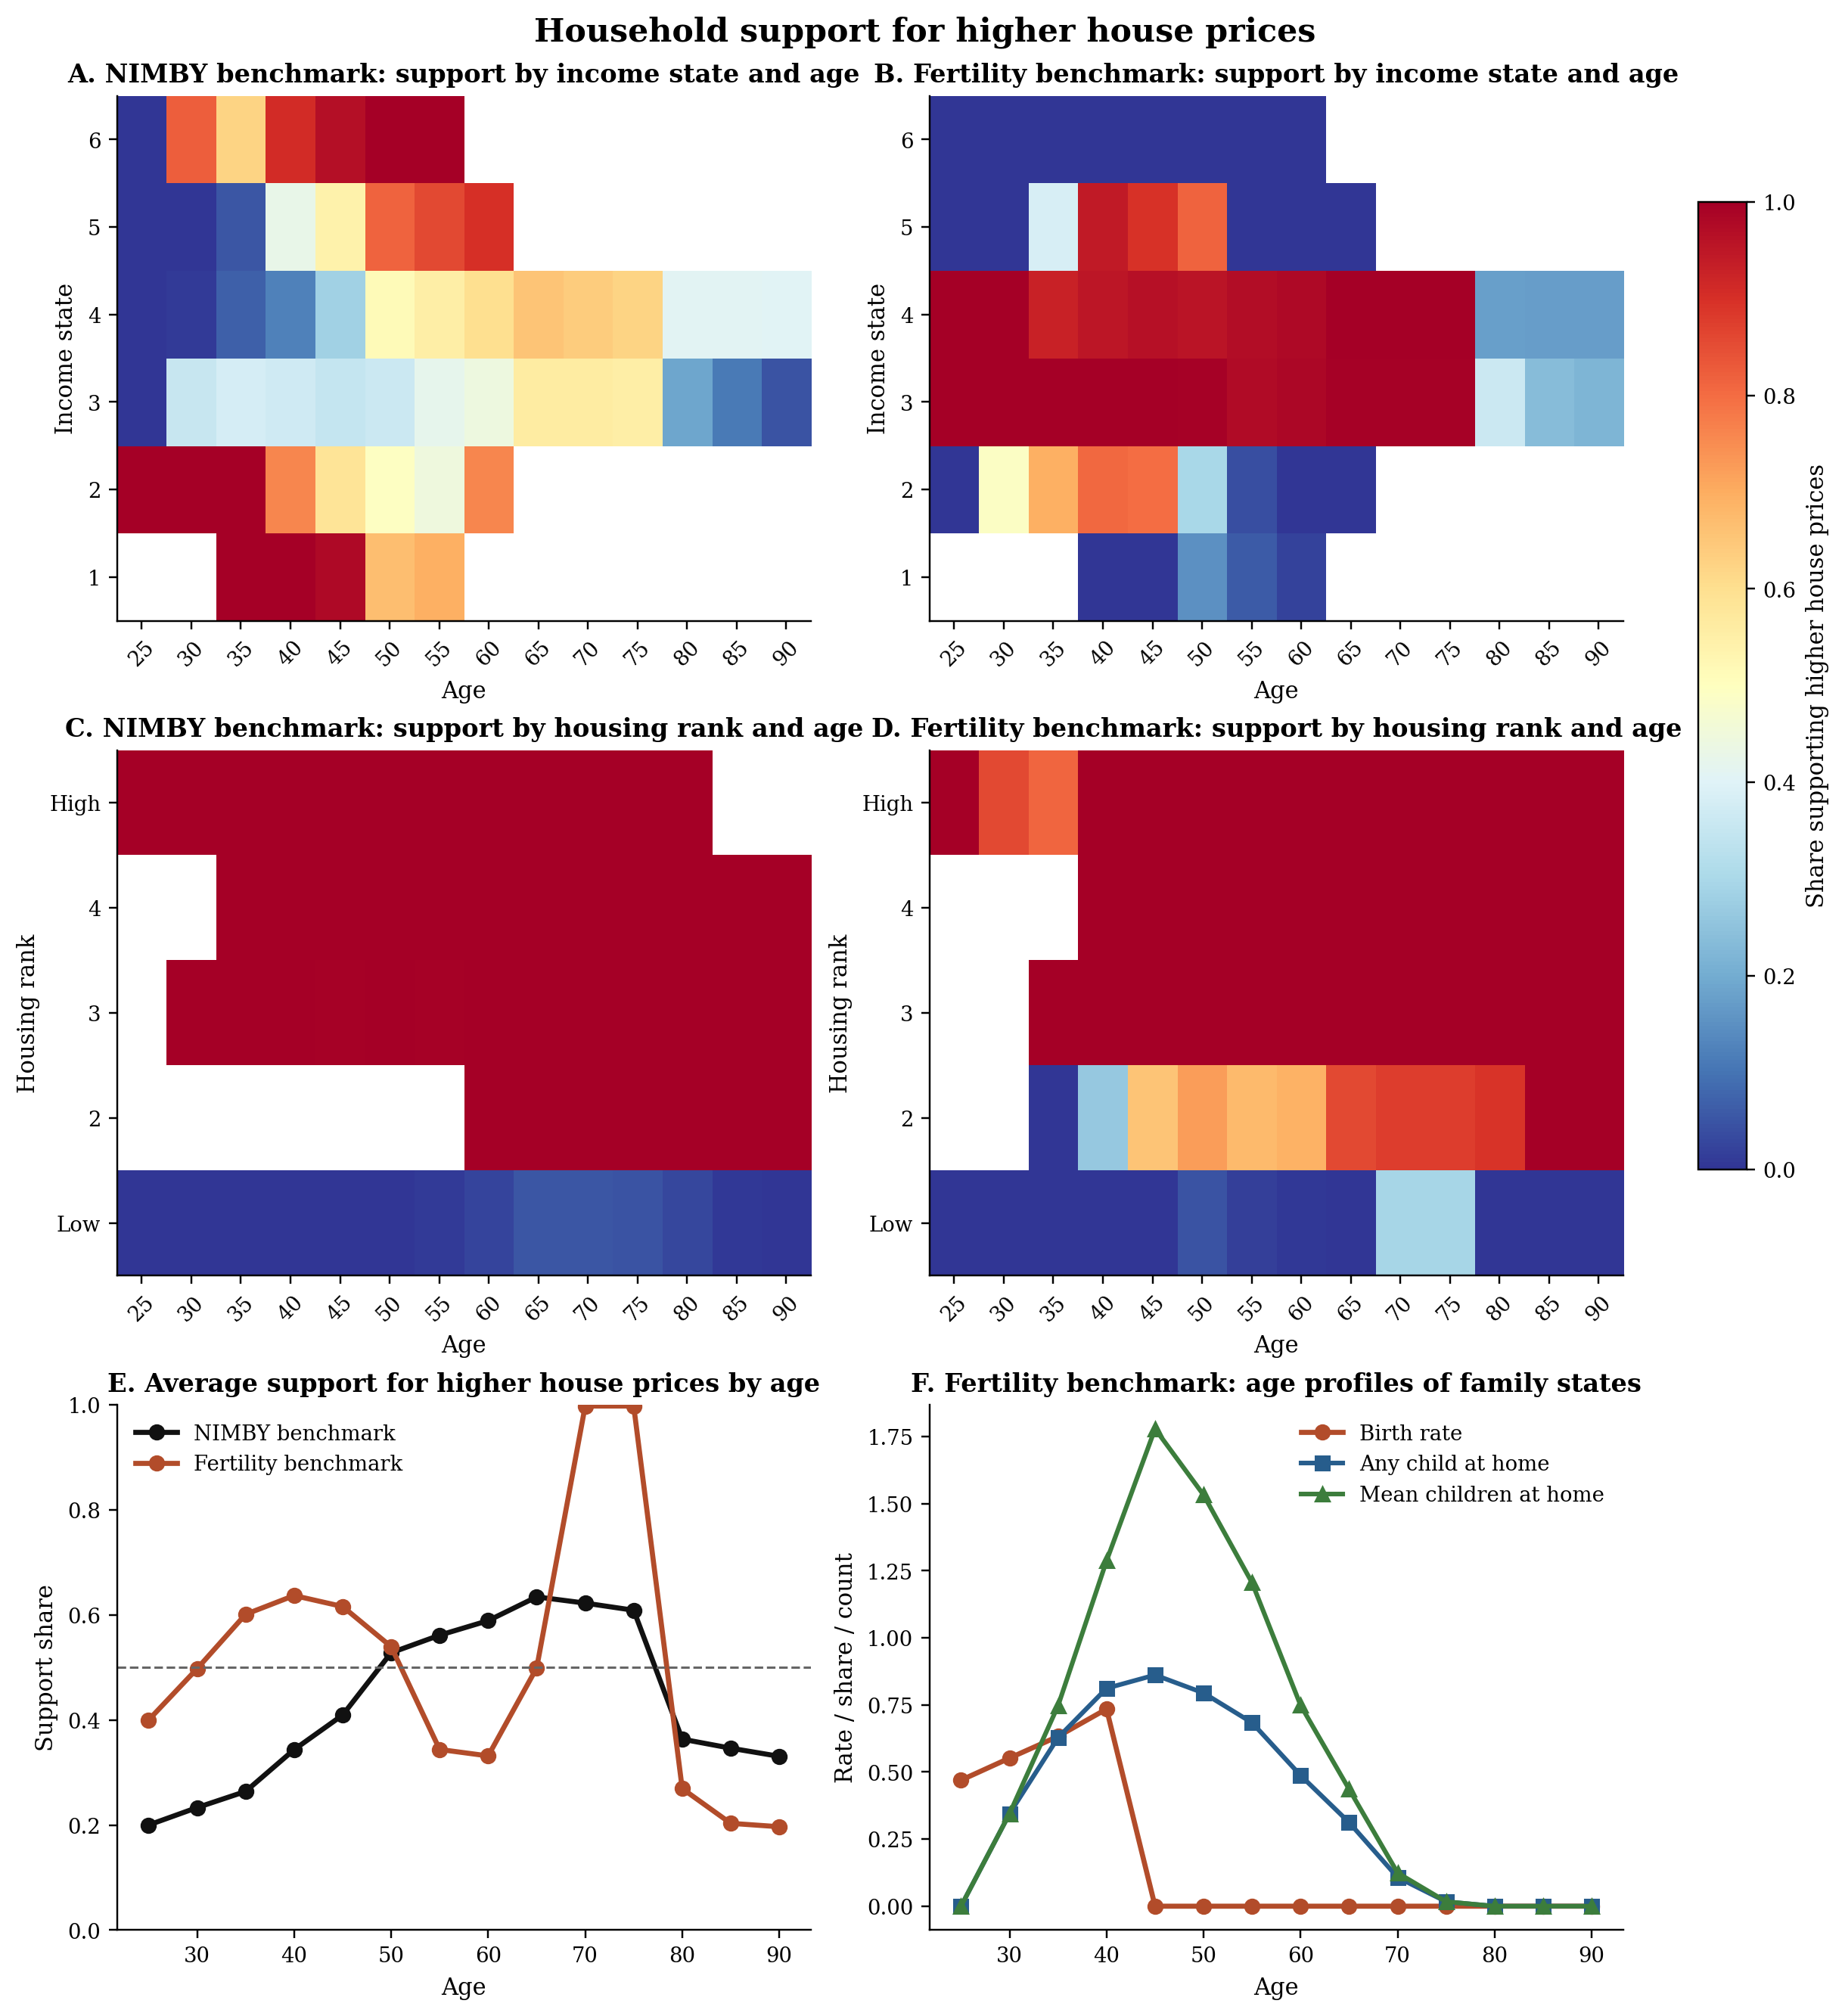
\includegraphics[width=\textwidth]{nimby_vs_fertility_household_support.png}
\caption{Household support for higher house prices in the NIMBY benchmark and the fertility
extension. The fertility model preserves the baseline age and tenure logic, but family states with
children at home are systematically less tolerant of high house prices.}
\label{fig:steady_state_support}
\end{figure}

\begin{figure}[htbp]
\centering
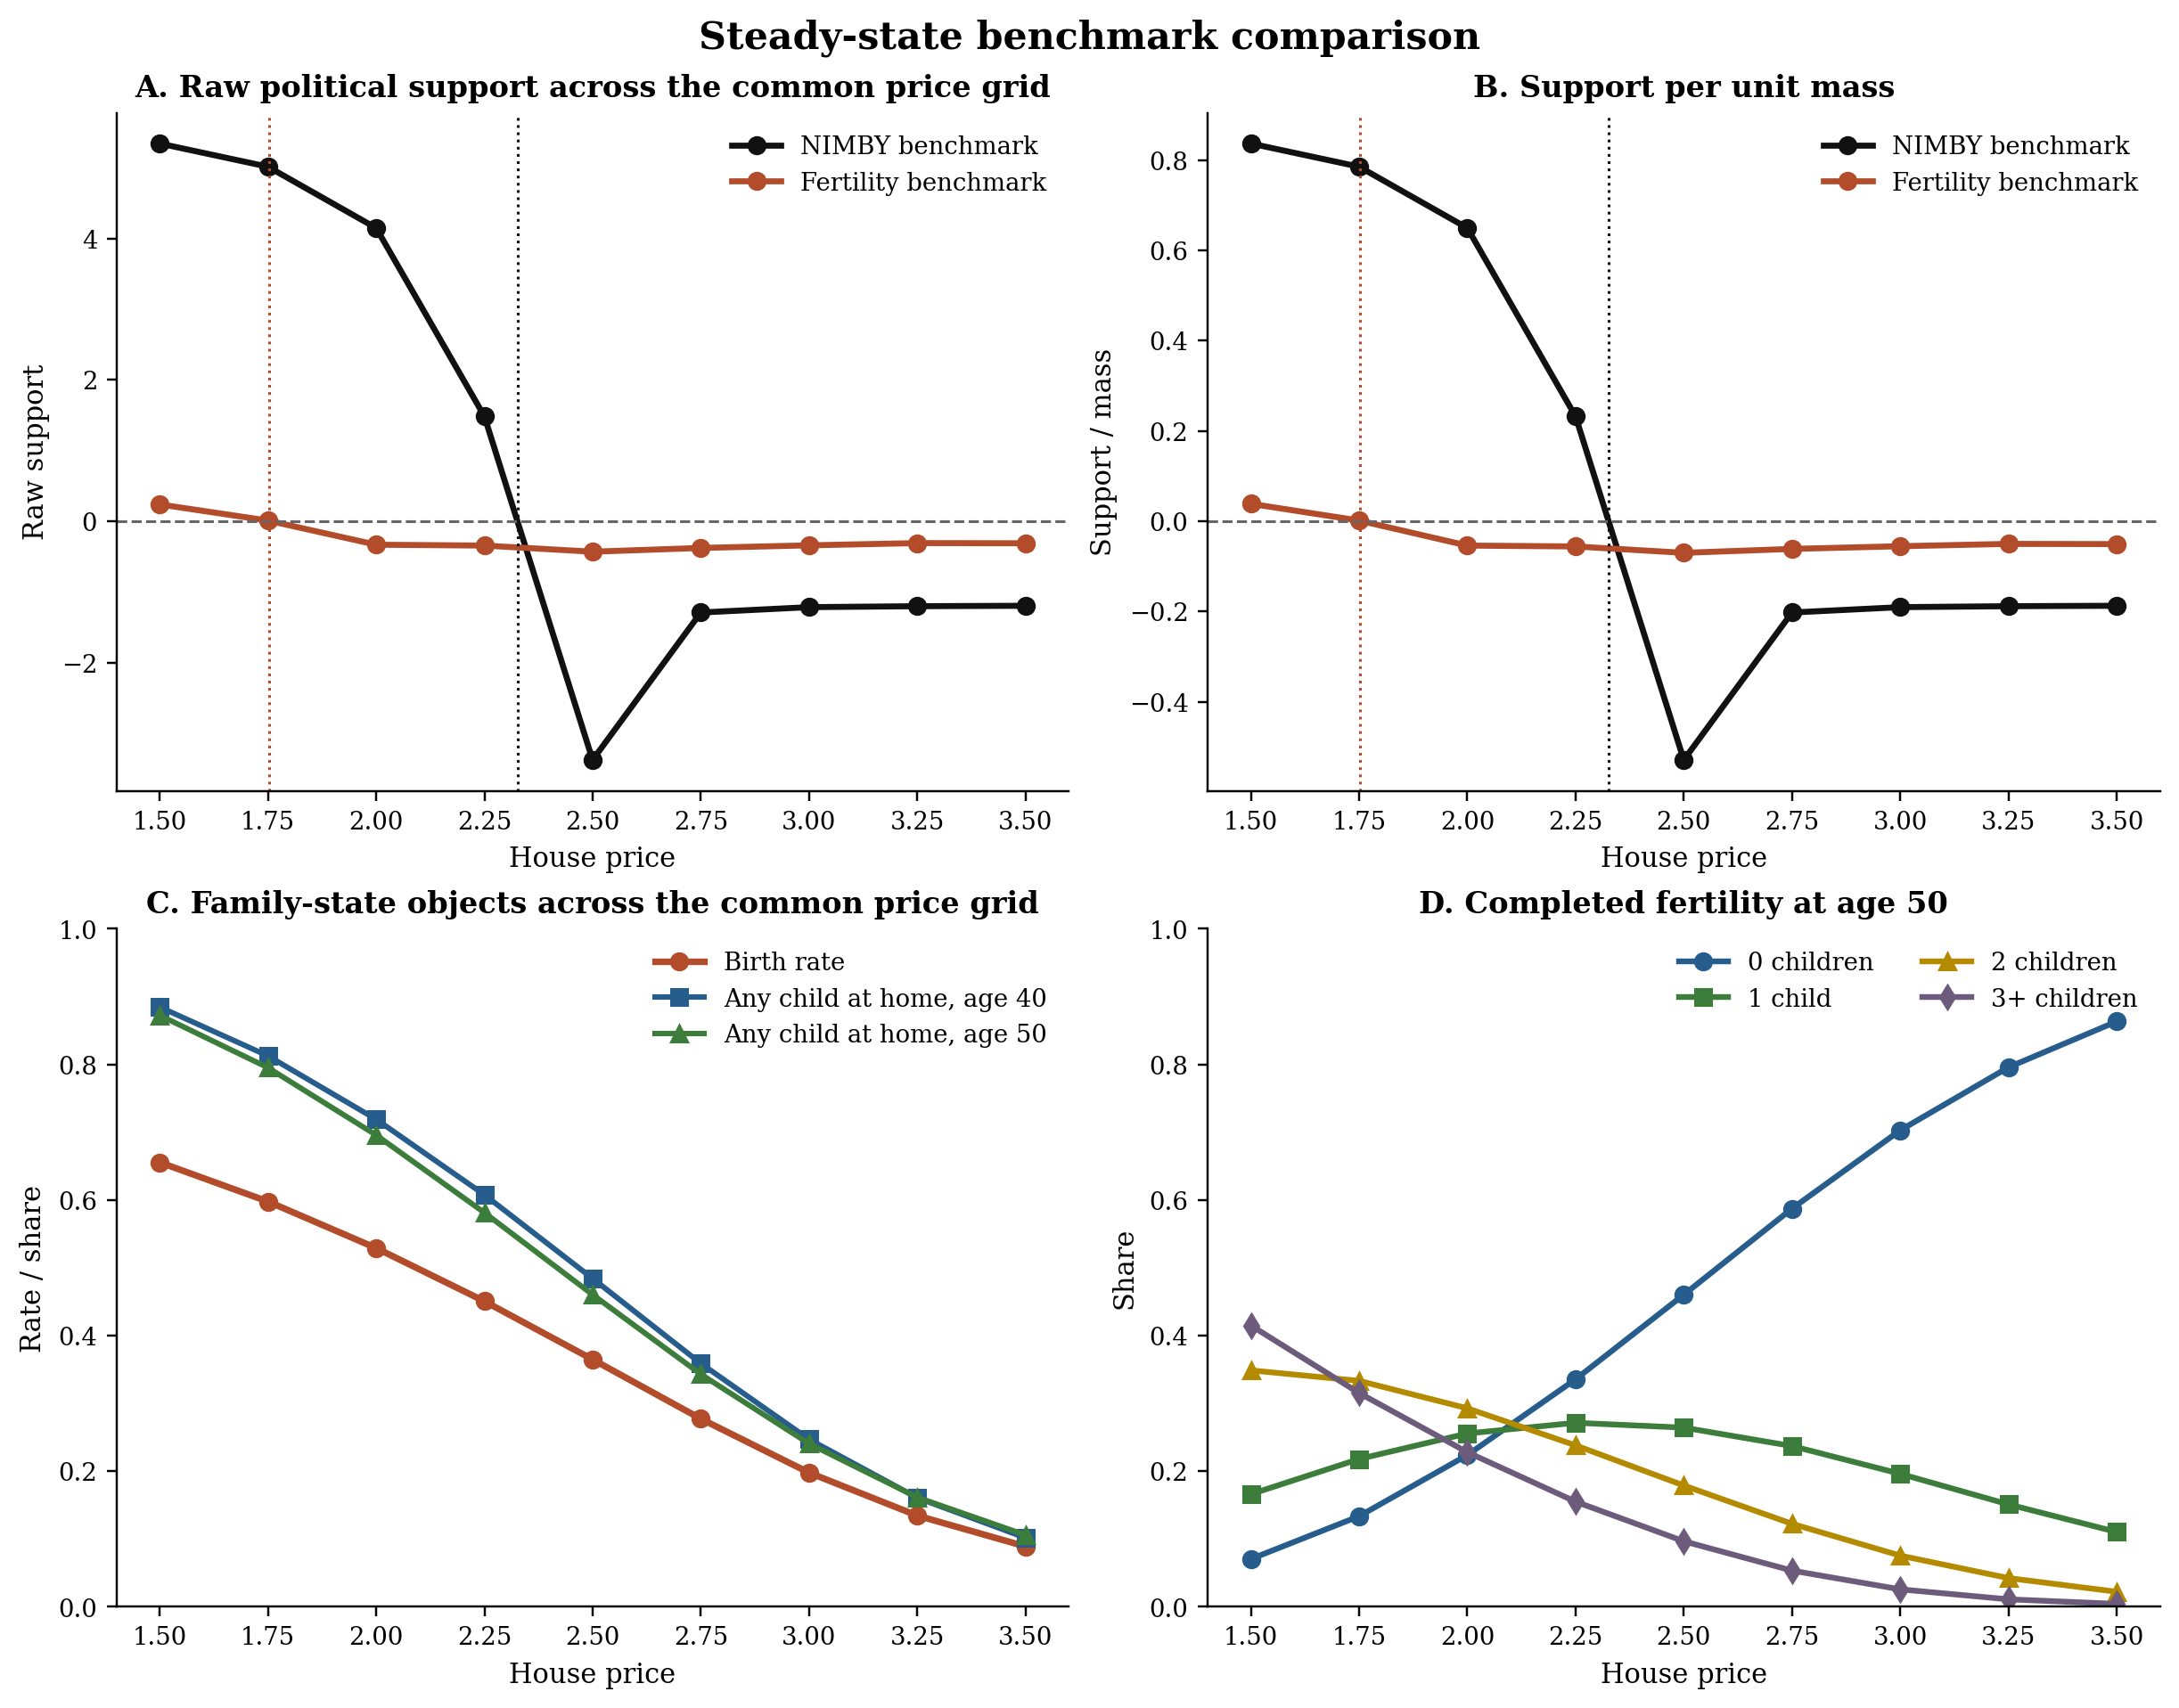
\includegraphics[width=\textwidth]{nimby_vs_fertility_benchmark_objects.png}
\caption{Steady-state benchmark comparison on the common house-price grid. The fertility extension
shifts the aggregate support schedule toward lower prices and changes family-state outcomes along
the grid.}
\label{fig:steady_state_objects}
\end{figure}

\section{A Temporary Baby Boom}

The next question is dynamic rather than static. What happens if births rise temporarily and the
large cohort moves through the life cycle? To make that comparison as close as possible to the
original NIMBY exercise, I impose the same temporary baby-boom shock used in the upstream
transition benchmark: a 10 percent increase in births for 10 periods.

The main result is that the fertility extension produces a larger medium-run house-price response
than the NIMBY benchmark under the same demographic shock. Figure \ref{fig:baby_boom} reports the
matched transition comparison. Normalizing each model by its own initial house-price level, the
average post-window price response is about 2.0 percent in the NIMBY transition and about 5.1
percent in the fertility transition.

That amplification comes from the family-demand channel. In the NIMBY benchmark, a baby boom works
mainly through cohort size and future political composition. In the fertility model, the same
shock also raises the stock of children at home. Those children make housing space more valuable
right away because crowding is costly. So the baby boom does more than create a larger future
cohort. It raises contemporaneous housing demand.

The family margin also creates a feedback that runs in the opposite direction later. In the
fertility transition, the fertility rate rises during the boom by about 0.022 relative to
baseline, then slips modestly below baseline later. High house prices therefore dampen future
fertility even while the initial child wave is amplifying current housing demand.

\begin{figure}[htbp]
\centering
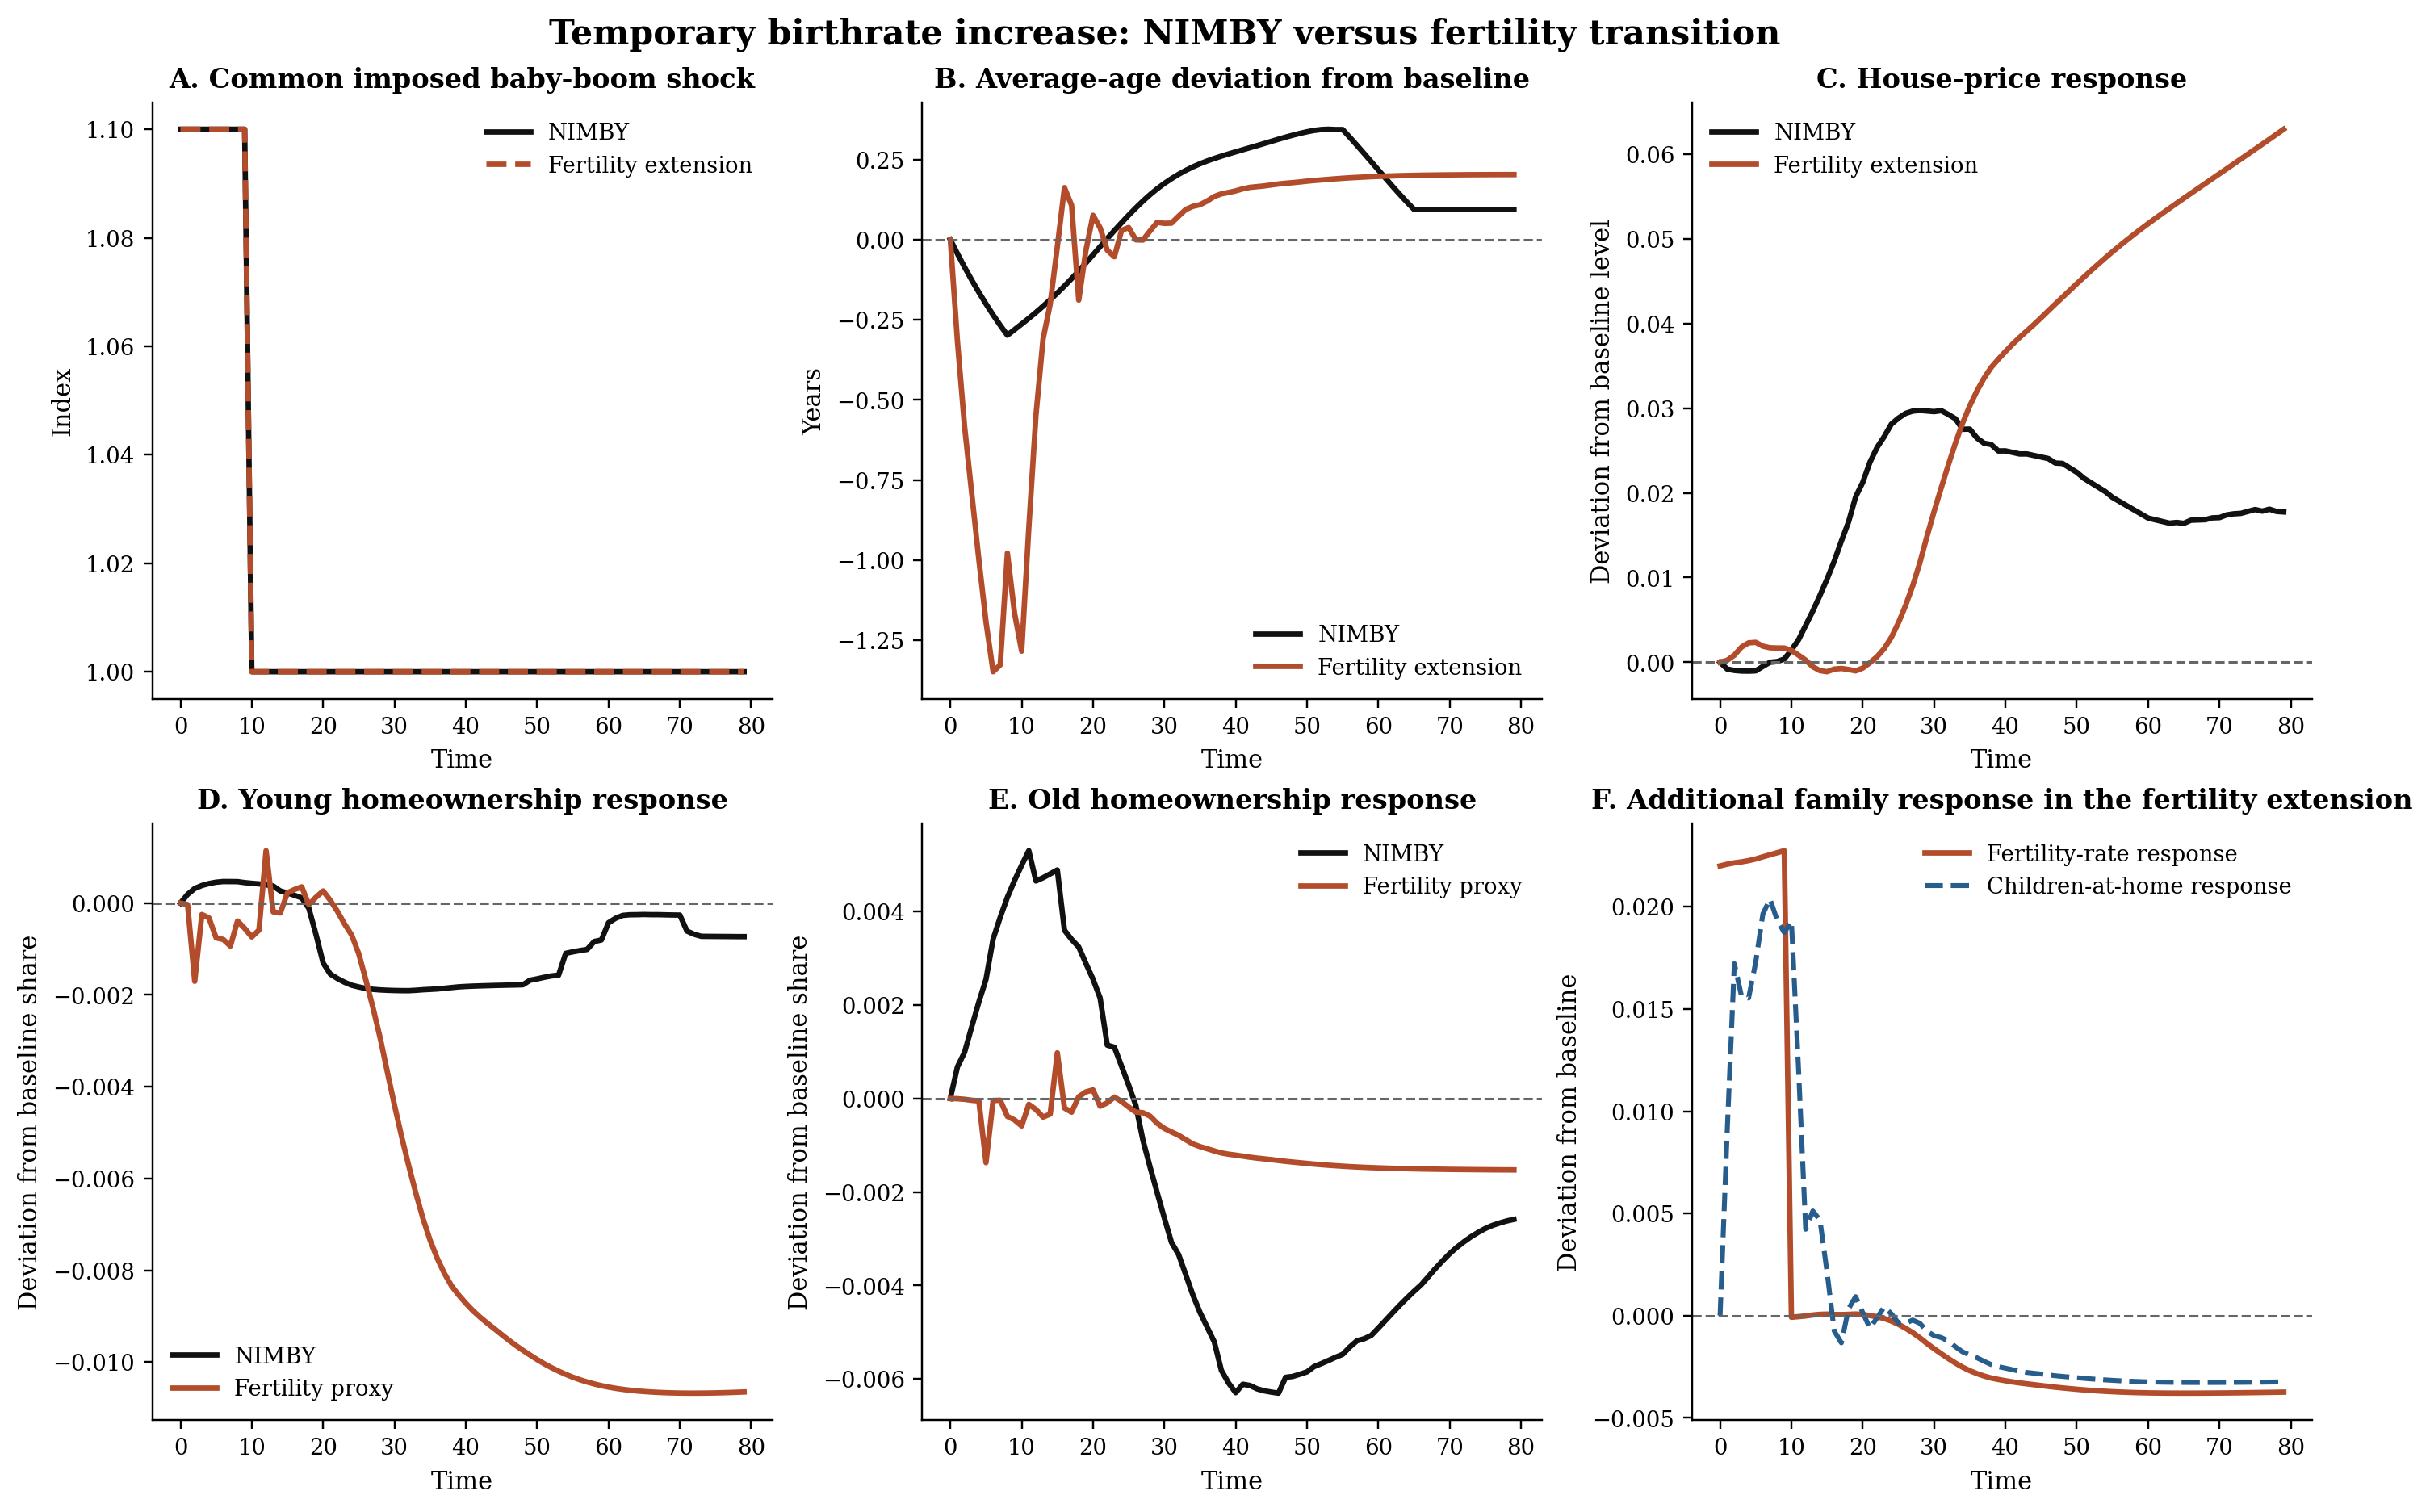
\includegraphics[width=\textwidth]{nimby_vs_fertility_baby_boom_transition.png}
\caption{Temporary birthrate increase: NIMBY versus fertility transition. The fertility extension
produces a larger medium-run house-price response than the NIMBY benchmark and introduces an
additional family-state response through births and children at home.}
\label{fig:baby_boom}
\end{figure}

Figure \ref{fig:cohort_access} reports the current cohort-incidence counterpart. The NIMBY lines
are the upstream cohort homeownership indices. The fertility lines are access proxies built from a
common age profile and the model-implied house-price path. They are not a structural tenure solve,
but they are informative about incidence. The child generation is hit hardest, the boom
generation next, and the parent generation least.

\begin{figure}[htbp]
\centering
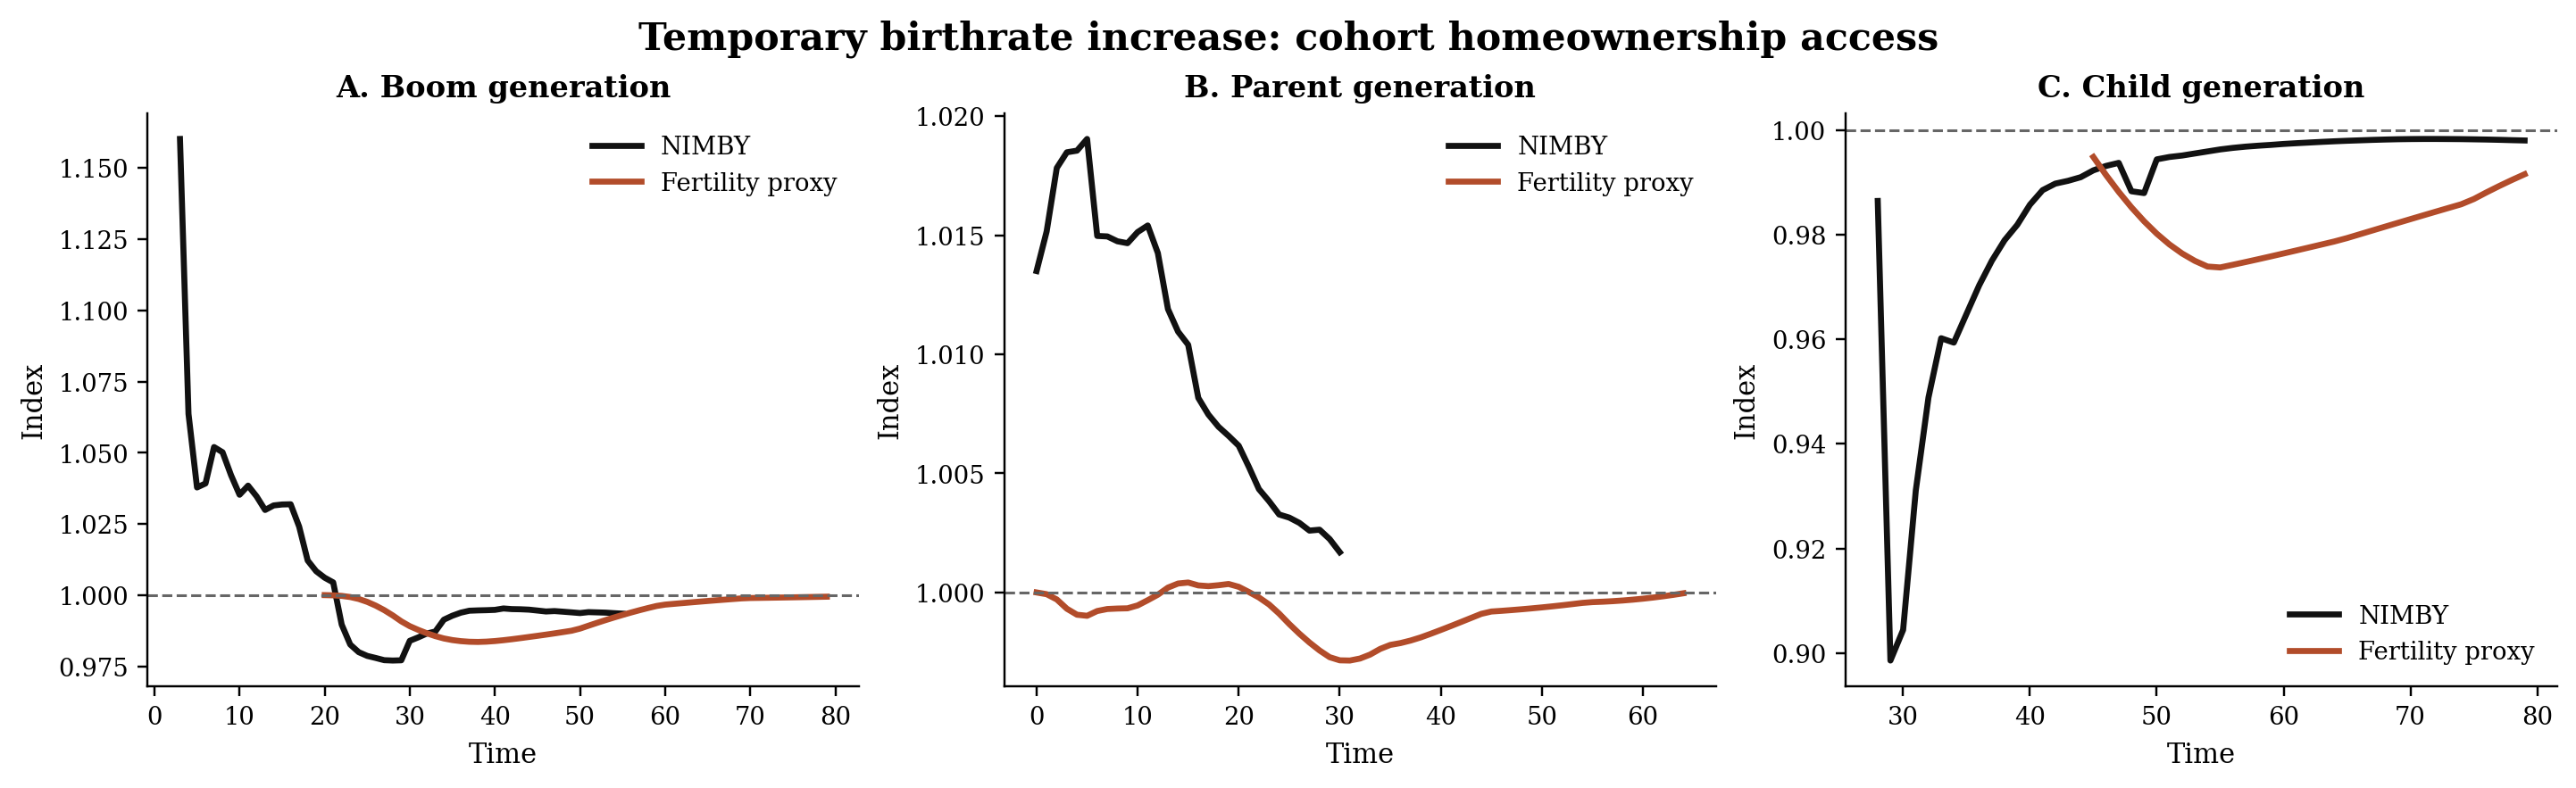
\includegraphics[width=\textwidth]{nimby_vs_fertility_generation_homeownership.png}
\caption{Temporary birthrate increase: cohort homeownership access. The black lines are the
upstream NIMBY indices. The red lines are fertility-side access proxies built from the matched
transition bridge.}
\label{fig:cohort_access}
\end{figure}

\section{Historical Validation}

The baby-boom experiment naturally raises a validation question. Does the fertility extension help
the model match the long decline in observed fertility after the postwar boom?

Figure \ref{fig:historical_validation} compares the model to the aggregate historical fertility
series from the legacy NIMBY data. Because the historical baby boom is more persistent than the
toy 10-period shock, the clean comparison is the shape of the decline after the boom rather than
exact calendar matching of the peak. Once the historical series is aligned at 1956 and the model
is aligned at period 10, the fertility extension fits the decline modestly better than the NIMBY
path at each horizon considered. The 10-year RMSE falls from 0.119 in NIMBY to 0.104 in the
fertility extension. The same ranking holds at 20, 30, and 40 years.

That is not a full quantitative validation. The historical decline is much larger and more
persistent than either model. But it is still informative. The original NIMBY transition has no
mechanism that can push fertility below baseline after the imposed baby-boom window ends. The
fertility extension does. On that margin, it moves the model in the right direction.

\begin{figure}[htbp]
\centering
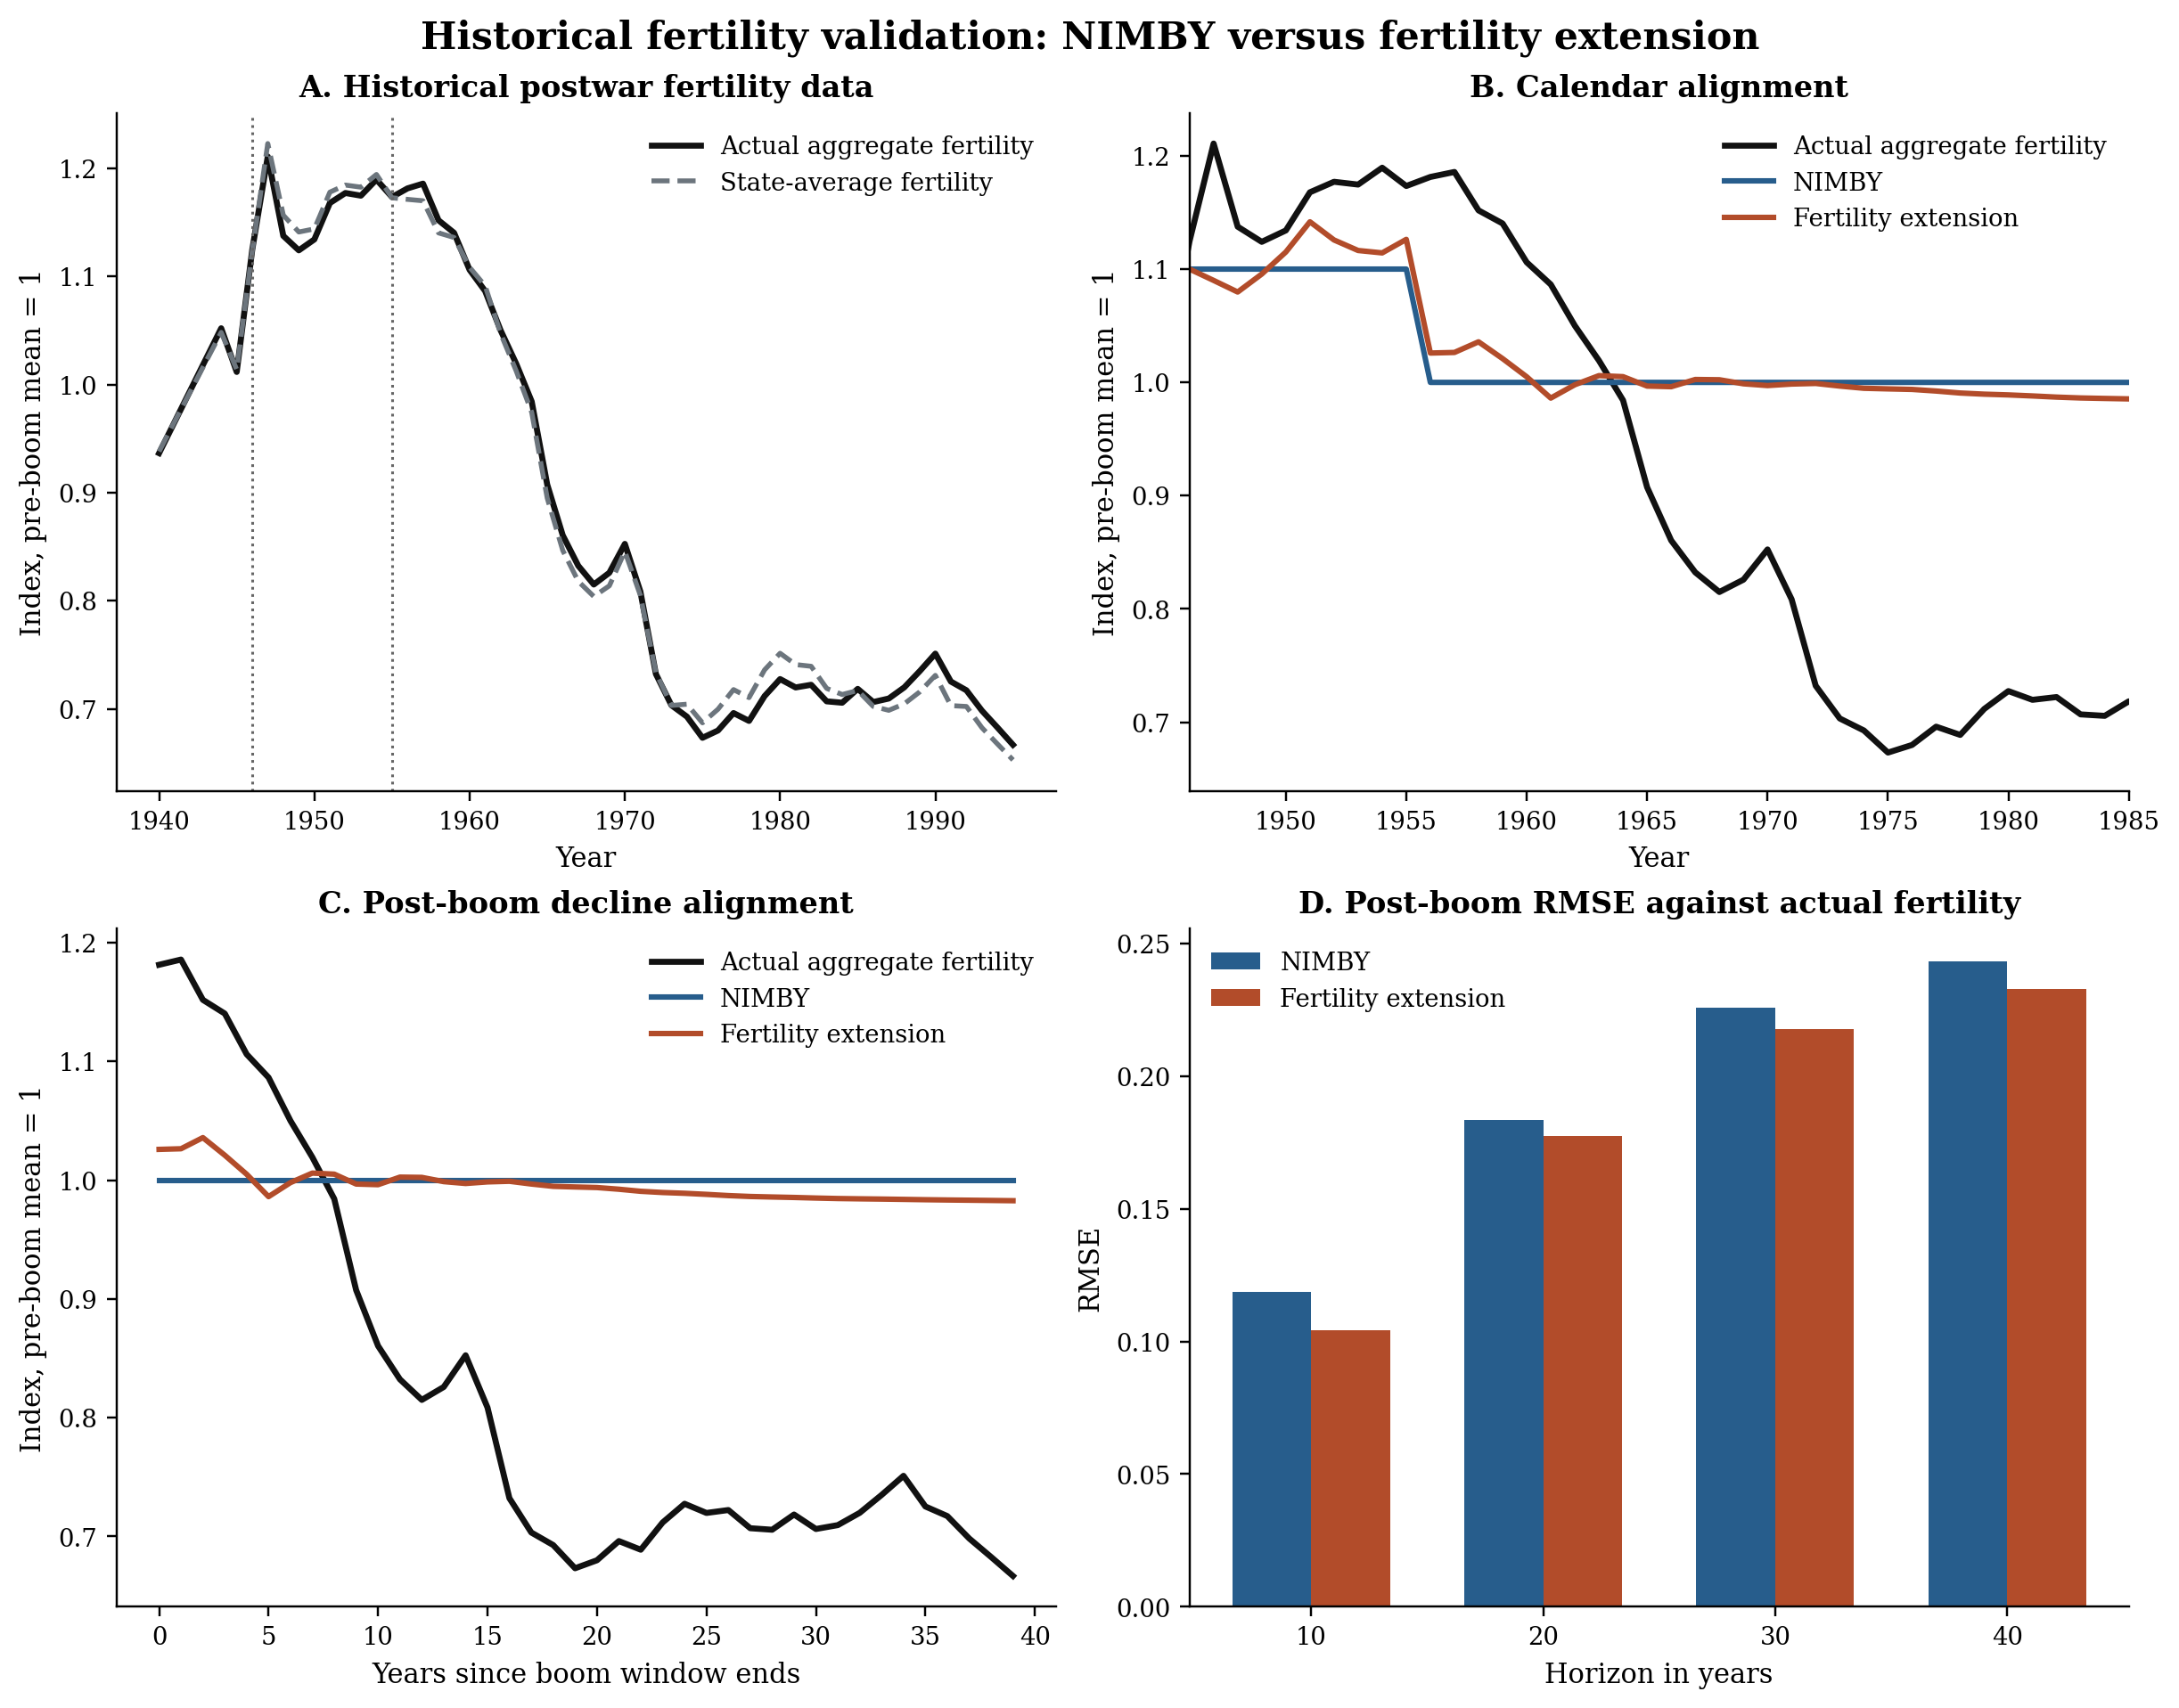
\includegraphics[width=\textwidth]{nimby_vs_fertility_historical_validation.png}
\caption{Historical fertility validation. The fertility extension fits the aligned post-boom
decline in the aggregate historical series modestly better than the flat NIMBY return path.}
\label{fig:historical_validation}
\end{figure}

\section{Robustness}

The next concern is whether the short-run price result is a knife-edge consequence of one
particular parameter choice. Figure \ref{fig:robustness} reports a bounded robustness exercise
around three margins: the size of the baby-boom shock, the reduced-form price sensitivity of
fertility, and the strength of family demand in the housing block.

The robust conclusion is the price result. Across all three shock sizes, the fertility extension
produces a larger post-boom price response than the NIMBY proxy. At the benchmark 10 percent
shock, the response is about 0.051 in the fertility model against about 0.031 in the NIMBY proxy.
At a 30 percent shock, the same comparison becomes roughly 0.125 against 0.058. Varying the
price sensitivity of fertility over the range 0.10 to 0.30 hardly changes that ranking. Varying
family-demand strength shifts levels more noticeably, but the fertility line remains above the
NIMBY line throughout.

The access results are less uniform. Stronger shocks make young-homeownership access worse in both
models, and for large enough shocks the fertility extension has the more negative young-access
trough. But when the change comes from stronger price sensitivity of fertility or stronger family
demand rather than a larger demographic shock, the fertility model partly self-corrects through
lower later births. So the cleanest robust result is the price amplification result, not a claim
that every access proxy always worsens in the fertility extension.

\begin{figure}[htbp]
\centering
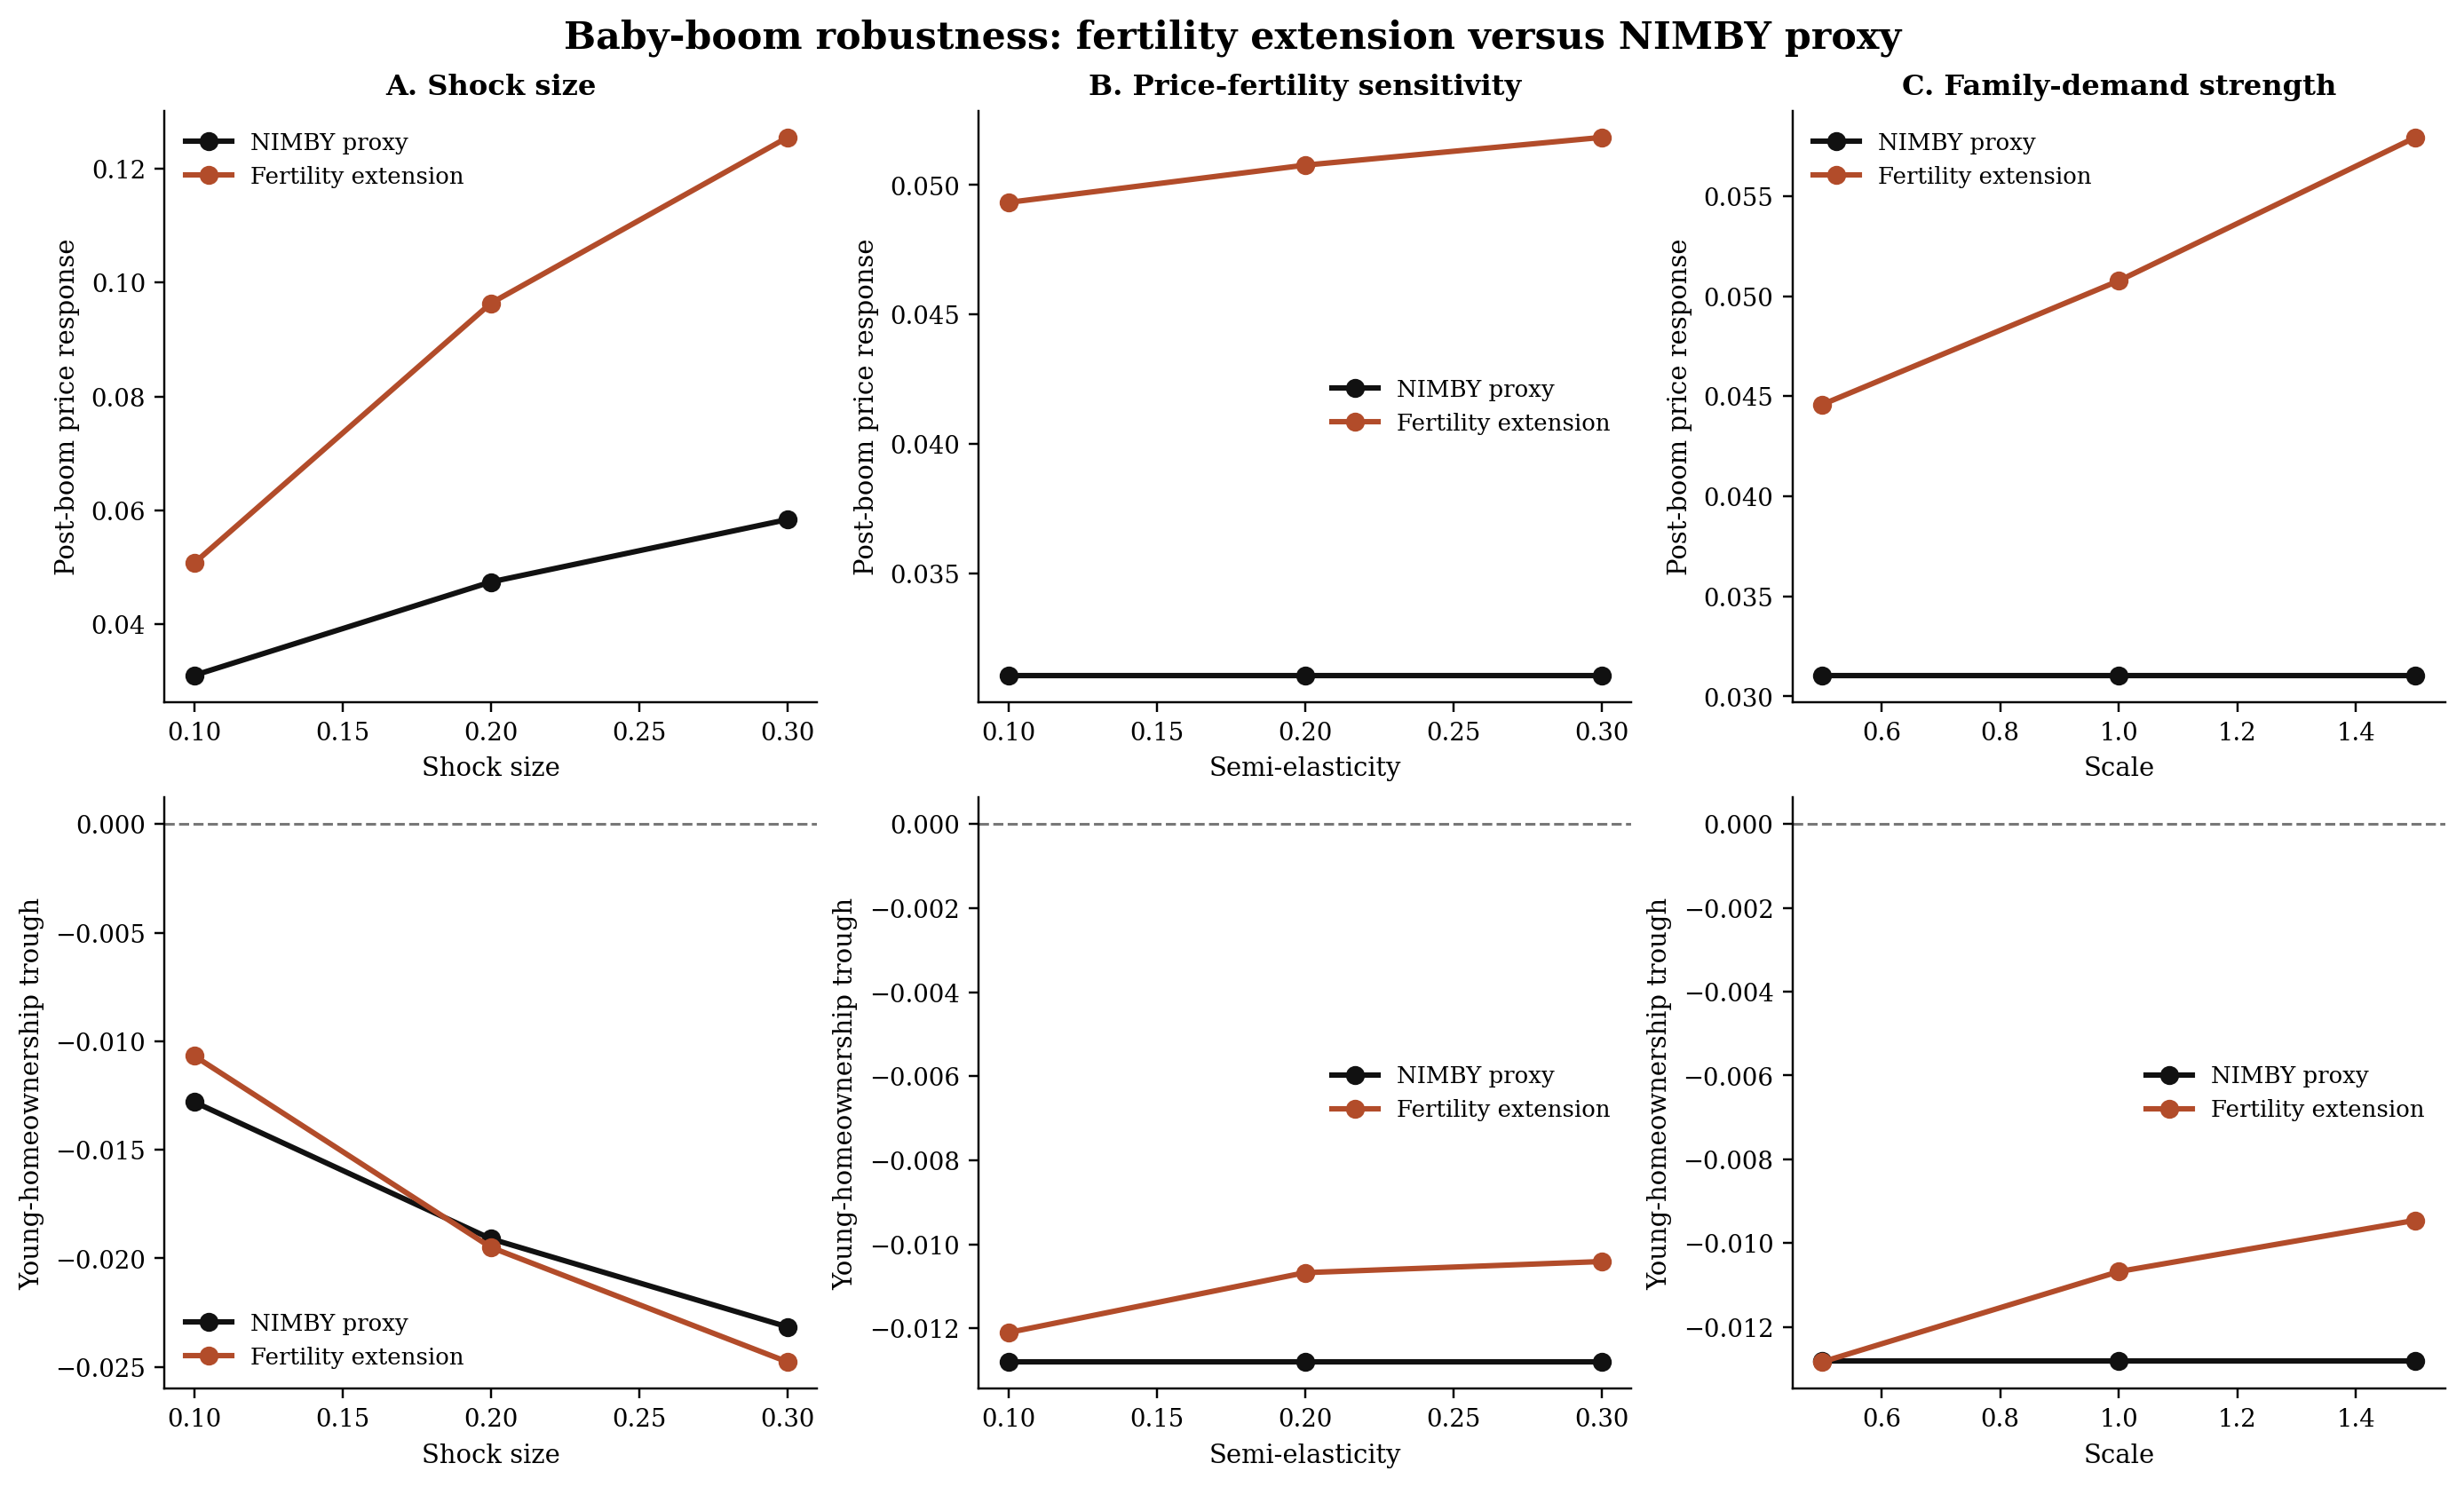
\includegraphics[width=\textwidth]{nimby_vs_fertility_transition_robustness.png}
\caption{Baby-boom robustness. The top row reports the post-boom house-price response. The bottom
row reports the young-homeownership trough. The price-amplification result is robust across the
bounded sweep.}
\label{fig:robustness}
\end{figure}

\section{Future Demographic Projections}

The NIMBY paper also studies long-run population aging. The natural question is whether the
fertility extension strengthens or weakens that forecast.

Figure \ref{fig:projection} feeds the same upstream projected age-weight scenarios into a matched
bridge exercise. The black line shuts off the fertility-demand channel and therefore plays the
role of the NIMBY side of the comparison. The red line keeps births and children at home in the
demand block. This is not yet the full project-02 forecast solver. It is a matched projection
bridge built from the forecast age scenarios. But it is still informative about the sign of the
fertility channel under projected aging.

The result goes in the opposite direction from the baby-boom impulse response. Under all three
immigration scenarios, projected aging raises the NIMBY proxy price path but leaves the fertility
path much flatter. In the medium-immigration scenario, the NIMBY proxy reaches a house-price
index of about 1.093 by 2050 and about 1.067 by 2100, while the fertility bridge is essentially
flat in 2050 and slightly below its 2020 level by 2100.

The interpretation is again economic rather than mechanical. In the baby-boom experiment, the key
family object is a temporary wave of children at home, which raises current space demand. In the
long-run aging exercise, the key family object is the shrinking mass of family-forming households.
That reduces the importance of the crowding channel. So the fertility extension dampens the
aging-driven rise in house prices rather than amplifying it.

\begin{figure}[htbp]
\centering
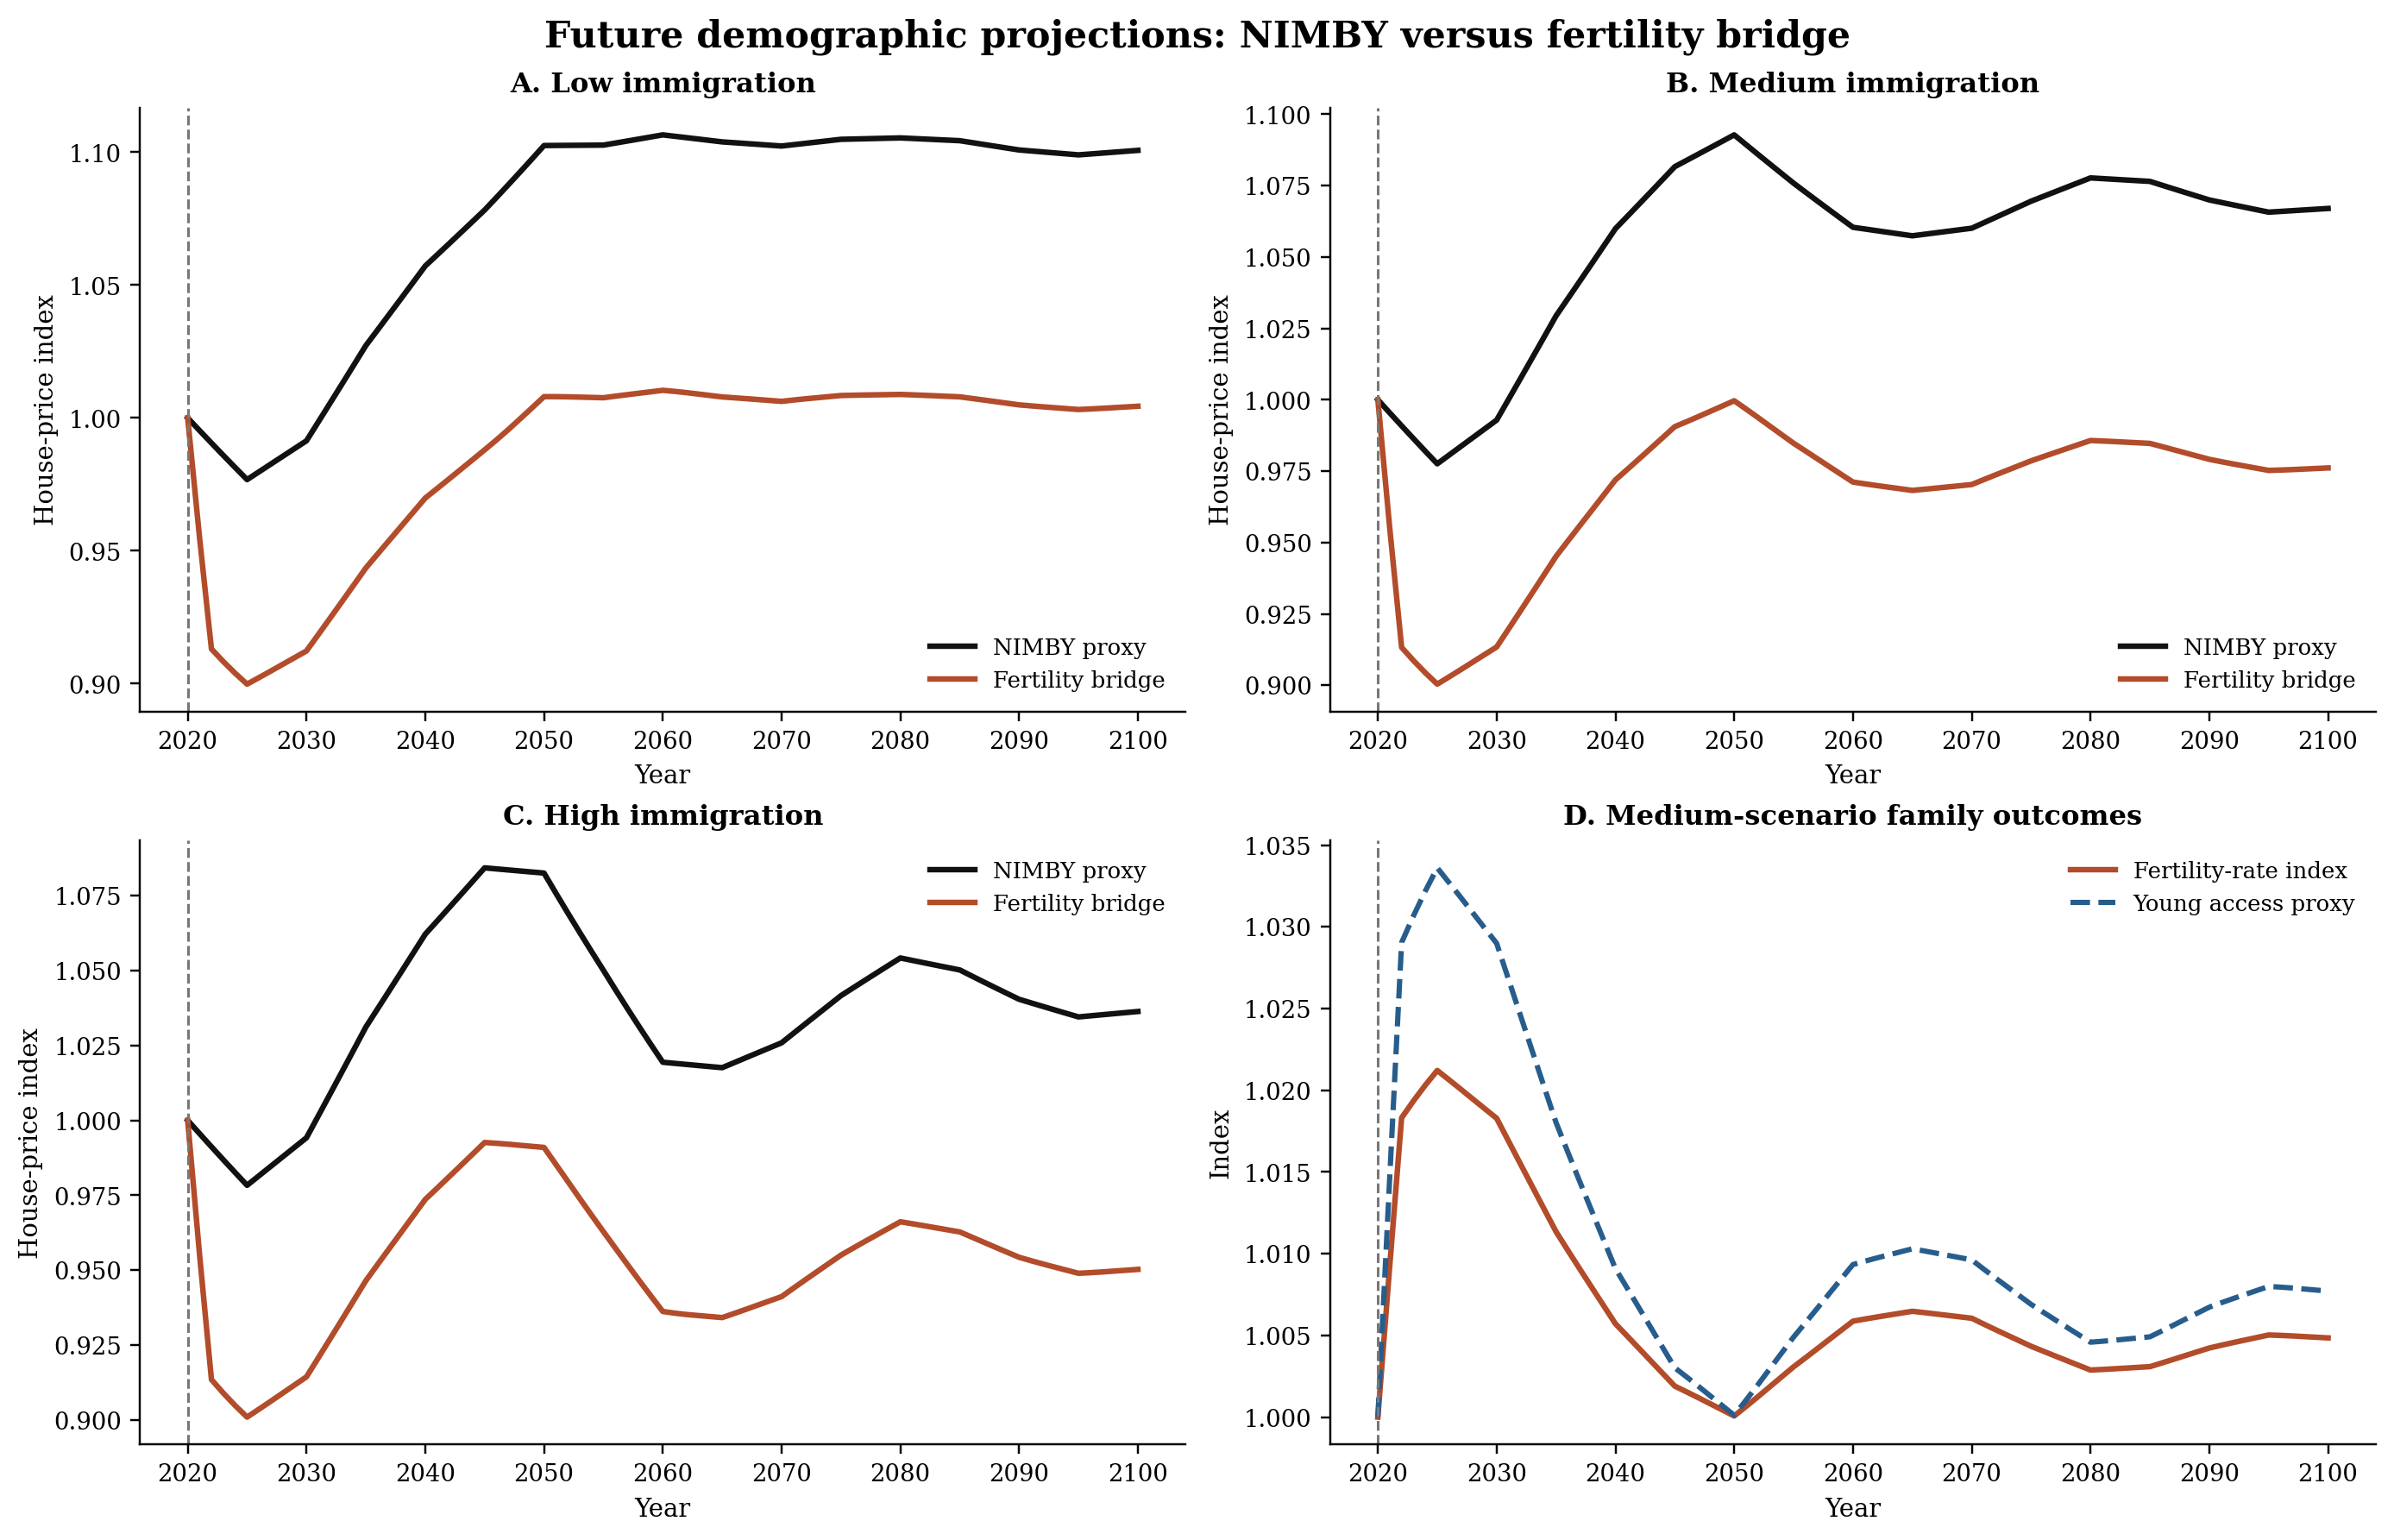
\includegraphics[width=\textwidth]{nimby_vs_fertility_projection_comparison.png}
\caption{Future demographic projections from the matched bridge. The fertility channel amplifies
the short-run child-wave experiment but tempers the long-run aging-driven rise in house prices.}
\label{fig:projection}
\end{figure}

\section{Conclusion}

The fertility model is not a different political model, a different housing-supply model, or a
different equilibrium concept. It is the NIMBY housing-supply model with an augmented household
problem in which births and children at home matter for the value of housing space.

That one change is enough to alter both the steady state and the transition dynamics. In the
steady state, the fertility channel shifts political support toward lower house prices. In a
temporary baby boom, it amplifies the medium-run house-price response because children at home
raise current housing demand. In the historical data, it improves the fit to the post-boom
fertility decline, though modestly. Under long-run projected aging, it works in the opposite
direction and dampens the rise in house prices relative to the NIMBY proxy.

Those results are enough to support a standalone model paper. The remaining missing objects are not
the basic comparison itself, but the richer savings, net-worth, and full forecast-solver layers
that would permit an exact one-for-one replication of every NIMBY figure. For the current paper,
the central model result is already clear: family formation changes the political economy of
housing supply in ways that the original NIMBY benchmark cannot capture.

\end{document}
